\documentclass[10pt]{article}
\usepackage[polish]{babel}
\usepackage[utf8]{inputenc}
\usepackage[T1]{fontenc}
\usepackage{amsmath}
\usepackage{amsfonts}
\usepackage{amssymb}
\usepackage[version=4]{mhchem}
\usepackage{stmaryrd}
\usepackage{graphicx}
\usepackage[export]{adjustbox}
\graphicspath{ {./images/} }

\begin{document}
\begin{enumerate}
  \item Dane są punkty A, B oraz przecinające się proste \(k\) i \(l\) (punkty A, B nie leżą na prostych \(k, l)\). Skonstruuj takie punkty C, D leżące odpowiednio na prostych \(k, l\), aby czworokąt ABCD był równoległobokiem. Podaj opis konstrukcji i uzasadnienie jej poprawności.\\
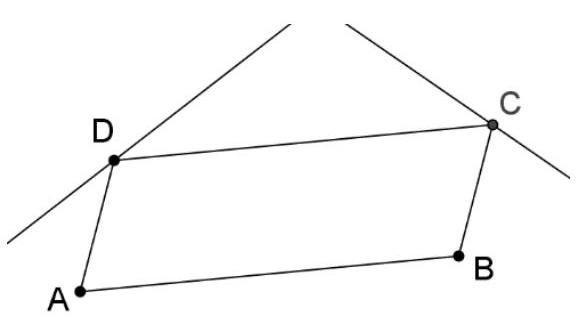
\includegraphics[max width=\textwidth, center]{2024_11_21_747b5439fbaad6f577a8g-1(1)}
  \item Odcinki czerwone mają długość 5 a odcinki niebieskie długość 3. Oblicz pole zacieniowanego obszaru.\\
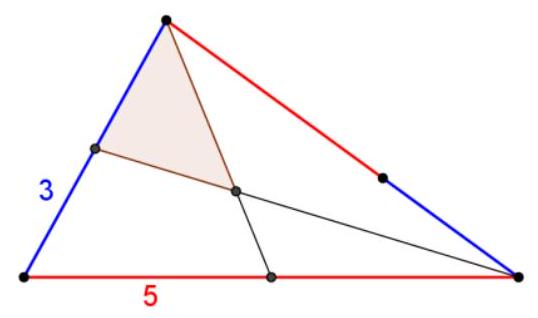
\includegraphics[max width=\textwidth, center]{2024_11_21_747b5439fbaad6f577a8g-1}
  \item Niech \(p\) będzie ustaloną liczbą pierwszą. Wyznacz wszystkie pary \((x, y)\) liczb całkowitych spełniających równanie
\end{enumerate}

\[
\frac{x y}{x+y}=p
\]


\end{document}